
\documentclass[12pt,a4paper]{article}
\usepackage[utf8]{inputenc}
\usepackage{graphicx}
\usepackage{float}
\usepackage{subcaption}
\usepackage{listings} % for code
\usepackage{color}
\usepackage{hyperref}    % can use url or hyperref package for url in bibtex
%% --- flow charts ----
\usepackage{adjustbox} 
\usepackage{tikz}
\usepackage{verbatim}
\usetikzlibrary{shapes.geometric, arrows}
    \tikzstyle{startstop} = [rectangle, rounded corners, minimum width=3cm, minimum height=1cm,text centered, draw=black]
    \tikzstyle{io} = [trapezium, trapezium left angle=70, trapezium right angle=110, minimum width=3cm, minimum height=1cm, text centered, draw=black] % ,fill=blue!30
    \tikzstyle{process} = [rectangle, minimum width=3cm, minimum height=1cm, text centered, draw=black, text width = 5cm]
    \tikzstyle{decision} = [diamond, node distance=3.5cm, minimum width=3cm, minimum height=5mm, text centered, draw=black, text width = 3cm,aspect=1.5]
    \tikzstyle{arrow} = [thick,->,>=stealth]
%% ----------------------------------------

\lstset{ % General setup for the package
	language=C++,
	basicstyle=\small\sffamily,
	numbers=left,
 	numberstyle=\tiny,
	frame=tb,
	tabsize=4,
	columns=fixed,
	showstringspaces=false,
	showtabs=false,
	keepspaces,
	commentstyle=\color{red},
	keywordstyle=\color{blue}
}
%% -------------------------------------------------------------------------
\title{ELP780 Software Lab\\Lab-2}
\author{Sah Swapnil Agrawal\\2018EET2554\\2018-20}
\date{\today}

\begin{document}
    \pagenumbering{gobble}
    \maketitle
    \begin{center}
    A report for the lab on C programming
    \end{center}
    \vspace{20pt}
    \begin{figure}[h!]
        \centering
        
\includegraphics{iitd_logo.jpg}
    \end{figure}
    \begin{center}
    \vspace{40pt}
    Department of Electrical Engineering\\
    IIT DELHI\\
    India
        
    \end{center}
    \newpage
    \tableofcontents
    \newpage
    \pagenumbering{arabic}
    \section{Problem Statement 1}
        \subsection{Problem statement}
        Consider a square matrix of size N(N x N matrix). Each element is of type unsigned integer.\\
        
        Let ri denote the minimum value in the i-th row, and ci denote the maximum value in i-th column. You have to obtain all such ri s and cis.\\From now on, let's call the set of all such ris ‘S1’, set of all cis ‘S2’ and set containing both ris and cis as ‘S’. i = 0 to N-1				 	 (20 min)
You have to do the following operations:
\begin{itemize}
\item From the set ‘S’, find the prime numbers and display those values on the terminal (10 min)
\item Consider string D as a concatenation of all the ris and cis e.g. If ‘S’ contains elements {13,10,5,7,10,7}, string D will become 131057107. \item Now substring will be entered by the user and the program should be able to find the position of the first occurrence of that substring in D. Display that position along with string D on the terminal. If the substring is not found then display the message stating no substring matched. 		(30 min)
\item Find the local minima and local maxima and display the index at which they occur in the set ‘S’. If no minima and maxima are found, display the message accordingly.		(30 min)
\end{itemize}

             \noindent We have to write a C program to perform some operations on the data obtained in a matrix format.
        \subsection{Assumptions}
            \noindent We are making no assumptions.
        \subsection{Algorithms and Implementation}
            \begin{itemize}
                \item Take the matrix as input from user.
                \item Find minimum element in each row and store these in set s1.
                    \begin{itemize}
                        \item Go to each row and take first element as the minimum element.
                        \item Start comparing this \textit{min} element with the other elements in the row.\\
                            If the \textbf{element} is smaller than \textit{min} then\\
                                assign this \textbf{element} to \textit{min}
                    \end{itemize}
                \item Find maximum element in each column and store these in set s2.
                    \begin{itemize}
                        \item Go to each column and take first element as the maximum element.
                        \item Start comparing this \textit{max} element with the other elements in the row.\\
                        If the \textbf{element} is greater than \textit{max} then\\
                                assign this \textbf{element} to \textit{max}
                    \end{itemize}
                \item Combine sets s1 and s2 to form set s.
                \item Find prime numbers in set s and display them.
                \item Create a string from the numbers in set s.
                \item Ask user for substring to search for.
                \item Find first index for occurrence of substring using windowing technique.
                \item If substring does not exist, display not found.
                \item Find local minima and local maxima in the set s. Note that first and last element do not come under local minima and local maxima.
                \item Display the local minima and local maxima as output.
            \end{itemize}

        \subsection{Input and Output format}
            \begin{itemize}
                \item \textbf{Input format}\\Input is given in the form of an NxN matrix with the order of matrix being given as command line argument
                \item \textbf{Output format}\\Output is displayed in the Terminal as per the problem statement.
            \end{itemize}
        \subsection{Test cases}
            ./ps1 4\\
            13 31 42 63\\
            90 41 31 52\\
            90 414 78 89\\ 
            9014 7582 980 7866\\

        \subsection{Difficulties /Issues faced}
            \begin{itemize}
                \item Difficulty faced in finding the presence of substring.
            \end{itemize}
        \subsection{Screenshots}
            \begin{figure}[H]
                \centering
                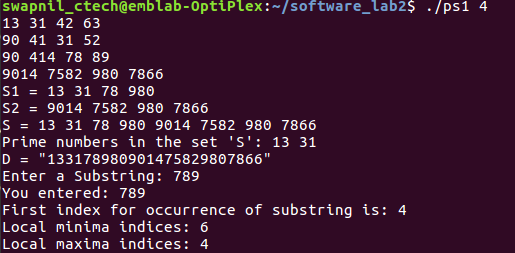
\includegraphics[width=\linewidth]{ps1.png}
                \caption{Output of program 1}
                \label{fig:my_label_1}
            \end{figure}
    \section{Problem Statement 2}
        \subsection{Problem statement}
            \paragraph{Split it Wisely!}
			Jeevan, Ramesh, Manisha, Parth and little chhaya went for a trip to Rishikesh. After returning from a trip, they are trying hard to split the expenses equally and settle their debts to each other. Help them splitting the expenses so that everyone gets to know how much money they owe to each other.\\
			We have to write a program for splitting the amount among people.
        \subsection{Assumptions}
            \begin{itemize}
                \item Name of the people is of max. length 100.
                \item The maximum length of purpose is 100.
                
            \end{itemize}
        \subsection{Algorithms and Implementation}
            \begin{itemize}
                \item Create a structure to hold the information about members.
                \item Take the name of members as input.
                \item Take the expense information from user as input.
                \item Ask user for choice of spltting.
                \item Split the amount based on the user's choice.
            \end{itemize}
        \subsection{Input and Output format}
            \begin{itemize}
                \item \textbf{Input format}\\Input is given in the form the names of members and then the expenses information and then the choice of method to split the money.
                \item \textbf{Output format}\\Output is shown in the Terminal as per problem statement.
            \end{itemize}
        \subsection{Test cases}
            ./ps2 4\\
    		akash\\
            swap\\
            aman\\
            deepak\\
            akash 2000 hotel\\
            akash 1000 min\\
            deepak 0 pizza\\
            swap 200 cap\\
            done\\
            4\\
            2 1 1 0\\
        \subsection{Difficulties /Issues faced}
            \begin{itemize}
                \item Creating the structure to store data.
                \item Calculating shares of each member.
                \item Determining whether float is required for amount.
            \end{itemize}
        \subsection{Screenshots}
            \begin{figure}[H]
                \centering
                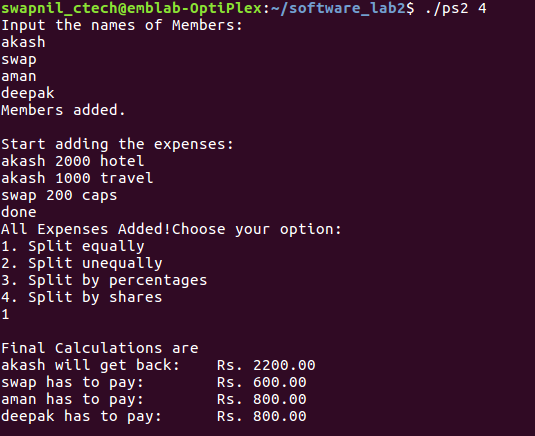
\includegraphics[width=\linewidth]{ps2_1.png}
                \caption{Output of program 2 with choice 1}
                \label{fig:my_label1}
            \end{figure}
            \begin{figure}[H]
                \centering
                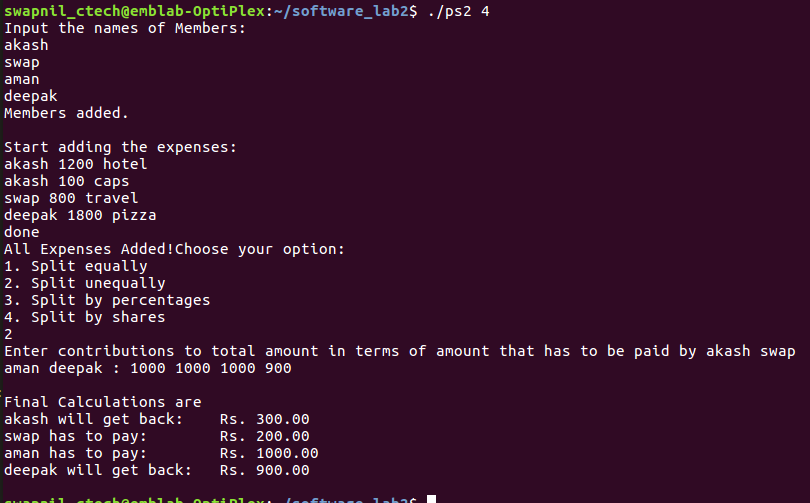
\includegraphics[width=\linewidth]{ps2_2.png}
                \caption{Output of program 2 with choice 2}
                \label{fig:my_label2}
            \end{figure}
            \begin{figure}[H]
                \centering
                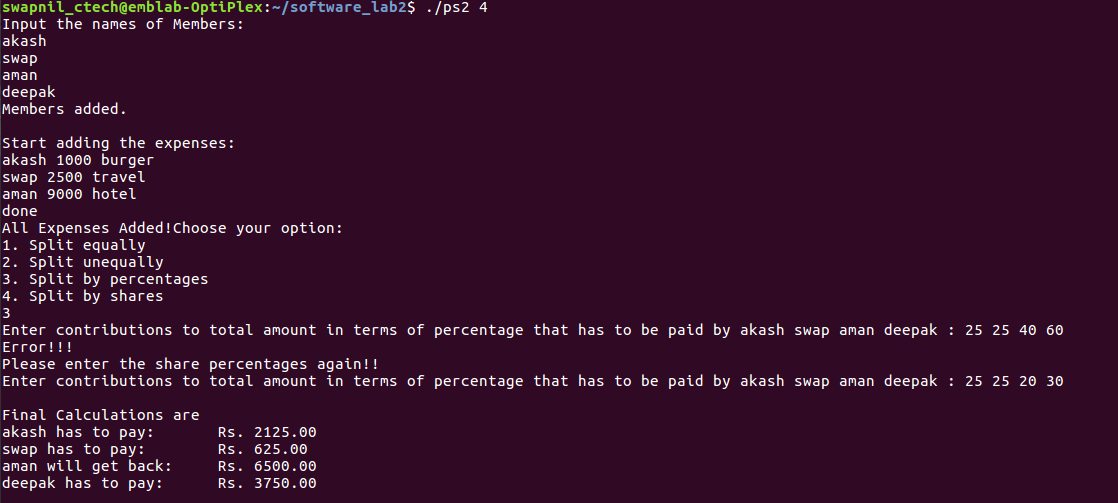
\includegraphics[width=\linewidth]{ps2_3.png}
                \caption{Output of program 2 with choice 3}
                \label{fig:my_label3}
            \end{figure}
            \begin{figure}[H]
                \centering
                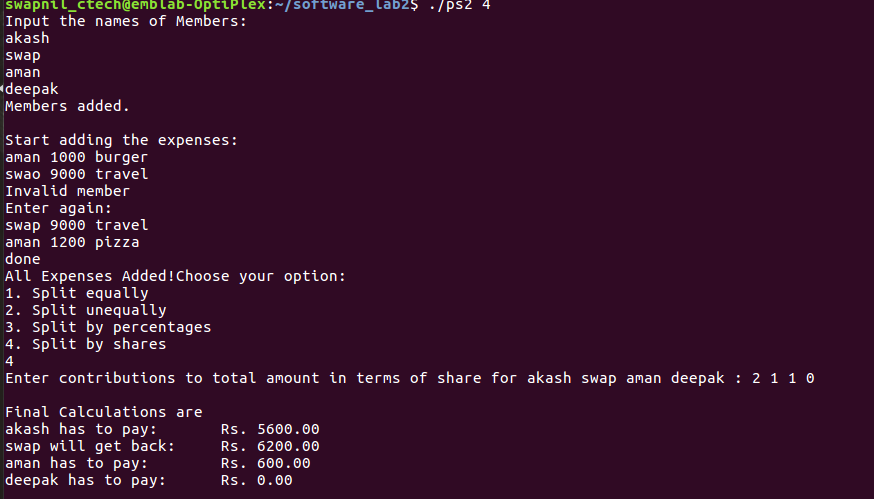
\includegraphics[width=\linewidth]{ps2_4.png}
                \caption{Output of program 2 with choice 4}
                \label{fig:my_label4}
            \end{figure}



    \newpage
    \section{Appendix}
        \subsection{Appendix A: Code for ps1}
            \verbatiminput{ps1.c}
        \subsection{Appendix B: Code for ps2}
            \verbatiminput{ps2.c}
    \newpage
    \nocite{*} %% use this if you want to add all fields in bibtex without citing anywhere
    \addcontentsline{toc}{section}{References}
    \bibliography{citations}
    \bibliographystyle{ieeetr}
\end{document}
